% first release v1.0, 20th October 1996
%       release v1.01, 29th October 1996
%       release v1.1, 25th June 1997
%   (based on JFMsampl.tex v1.3 for LaTeX2.09)
% Copyright (C) 1996, 1997 Cambridge University Press

\listfiles
\NeedsTeXFormat{LaTeX2e}

\documentclass{article}
\newcommand{\intinf} {\int\limits^{+\infty}_{-\infty}}
\newcommand{\eps} {$\varepsilon$}
\newcommand{\vfi} {$\varphi$}
\newcommand{\real} {I{\hspace{-1.4mm}}R}
\newcommand{\avektor} {a{\hspace{-3.0mm}}{\vspace{8mm}}\rightarrow}
\newcommand{\intRn} {\int\limits_{{I{\hspace{-1.1mm}}R}^n}}
\newcommand{\intRc} {\int\limits_{{I{\hspace{-1.1mm}}R}^3}}
\newcommand{\bA} {{\bf A}}
\newcommand{\bJ} {{\bf J}}
\newcommand{\bx} {{\bf x}}
\newcommand{\by} {{\bf y}}
\newcommand{\bz} {{\bf z}}
\newcommand{\bF} {{\bf F}}
\newcommand{\bff} {{\bf f}}
\newcommand{\bgg} {{\bf g}}
\newcommand{\bG} {{\bf G}}
\newcommand{\bh} {{\bf h}}
\newcommand{\bk} {{\bf k}}
\newcommand{\bl} {{\bf l}}
\newcommand{\ik} {{\it k}}
\newcommand{\nk} {\|{\bf k}\|}
\newcommand{\bxi} {{\mbox{\boldmath$\xi$}}}
\newcommand{\bn} {{\bf n}}
\newcommand{\bm} {{\bf m}}
\newcommand{\br} {{\bf r}}
\newcommand{\bs} {{\bf s}}
\newcommand{\bS} {{\bf S}}
\newcommand{\bv} {{\bf v}}
\newcommand{\bV} {{\bf V}}
\newcommand{\bw} {{\bf w}}
\newcommand{\bW} {{\bf W}}
\newcommand{\bu} {{\bf u}}
\newcommand{\bU} {{\bf U}}
\newcommand{\matS} {\mathcal{S}}
\newcommand{\matO} {\mathcal{O}}
\newcommand{\vecnab} {\vec{\nabla}}
\newcommand{\bvx} {\vec{\bf x}}
\newcommand{\bvy} {\vec{\bf y}}
\newcommand{\bvk} {\vec{\bf k}}
\newcommand{\etab} {{\bf \eta}}
\newcommand{\duzd} {{\mbox{d}}}
\newcommand{\duzn} {{\mbox{n}}}
\newcommand{\duzx} {{\mbox{x}}}
\newcommand{\duzy} {{\mbox{y}}}
\newcommand{\duzz} {{\mbox{z}}}
\newcommand{\duzS} {{\mbox{S}}}
\newcommand{\xxi} {x_{\xi}}
\newcommand{\xeta} {x_{\eta}}
\newcommand{\xzeta} {x_{\zeta}}
\newcommand{\yxi} {y_{\xi}}
\newcommand{\yeta} {y_{\eta}}
\newcommand{\yzeta} {y_{\zeta}}
\newcommand{\zxi} {z_{\xi}}
\newcommand{\zeeta} {z_{\eta}}
\newcommand{\zzeta} {z_{\zeta}}
\newcommand{\ve} {\vec{e}}
\newcommand{\vxxi} {\vec{x}_{\xi}}
\newcommand{\vxeta} {\vec{x}_{\eta}}
\newcommand{\vxzeta} {\vec{x}_{\zeta}}
\newcommand{\vyxi} {\vec{y}_{\xi}}
\newcommand{\vyeta} {\vec{y}_{\eta}}
\newcommand{\vyzeta} {\vec{y}_{\zeta}}
\newcommand{\vzxi} {\vec{z}_{\xi}}
\newcommand{\vzeta} {\vec{z}_{\eta}}
\newcommand{\vzzeta} {\vec{z}_{\zeta}}
\newcommand{\pp} [2] {\partial#1 \over \partial#2}
\newcommand{\ppy} [1] {\partial \over \partial#1}
\newcommand{\ppi} [2] {\partial^2#1 \over \partial#2^2}
\newcommand{\ppu} [3] {\partial^#1#2 \over \partial#3^#1}
\newcommand{\ppm} [3] {\partial^2#1 \over \partial#2\partial#3}
\newcommand{\ppd} [2] {\partial#1 / \partial#2}
\newcommand{\ppdu} [3] {\partial^#1#2 / \partial#3^#1}
\newcommand{\ppdm} [3] {\partial^2#1 / \partial#2\partial#3}
\newcommand{\DD} [2] {D#1 \over D#2}
\newcommand{\dd} [2] {d #1 \over d #2}
\newcommand{\ddu} [3] {d^{#1} #2 \over d #3^{#1}}
\newcommand{\Red}[1]{\textcolor[named]{Red}{#1}}
\newcommand{\Green}[1]{\textcolor[named]{Green}{#1}}
\newcommand{\Blue}[1]{\textcolor[named]{Blue}{#1}}
\newcommand{\boxed}[1]{\fbox{$ \displaystyle #1 $}}
\newcommand{\nin} {\in\hspace{-3mm}/}
\newcommand{\no}{\noindent}
\newcommand{\yes}{\indent}
\newcommand{\me}[3]{#1 \ddot{x} + #2\dot{x} + #3x}
\newcommand{\waveeqn} [2] {{1 \over #1^2}{\ppu{2}{#2}{t}}-\nabla^2{#2}}
\newcommand{\cwaveeqn} [2] {{\ppu{2}{#2}{t}}-#1^2\nabla^2{#2}}
\newcommand{\owaveeqn} [3] {{1 \over #1^2}{\ppu{2}{#2}{t}}-{\ppu{2}{#2}{#3}}}
\newcommand{\ocwaveeqn} [3] {{\ppu{2}{#2}{t}}-#1^2{\ppu{2}{#2}{#3}}}
\newcommand{\helm} [1] {\left(\nabla^2 + #1^2 \right)}
\newcommand{\ssum} [2] {\sum\limits_{#1}^{#2}}


% symbol fonts ...
% to be used with .. \usepackage{amsbsy}
\DeclareSymbolFont{AMSb}{U}{msb}{m}{n}
\DeclareMathSymbol{\N}{\mathbin}{AMSb}{"4E}
\DeclareMathSymbol{\Z}{\mathbin}{AMSb}{"5A}
\DeclareMathSymbol{\R}{\mathbin}{AMSb}{"52}
\DeclareMathSymbol{\Q}{\mathbin}{AMSb}{"51}
\DeclareMathSymbol{\I}{\mathbin}{AMSb}{"49}
\DeclareMathSymbol{\C}{\mathbin}{AMSb}{"43}

%----------------------------------------------------------------
%    commando \alpheqn voegt letters aan het formule-nummer
%    toe, (bijvoorbeeld 1.35a, 1.35b) en houdt het nummer gelijk,
%    tot het commando \reseteqn aangeroepen wordt

%\newcounter{saveeqn}%
%\newcommand{\alpheqn}{\setcounter{saveeqn}{\value{equation}}%
%\stepcounter{saveeqn}\setcounter{equation}{0}%
%\renewcommand{\theequation}
%    {\mbox{\arabic{chapter}.\arabic{saveeqn}-\alph{equation}}}}%
%\newcommand{\reseteqn}{\setcounter{equation}{\value{saveeqn}}%
%\renewcommand{\theequation}{\arabic{chapter}.\arabic{equation}}}%
%%%%%%%
% List with a diamond
\newcommand{\li}[1]{\item{#1}}
\newcommand{\bdli}[0]{
                     \begin{list}{$\diamond$}
                     {\setlength{\parsep}{0.0ex plus2.0ex}
                      \setlength{\topsep}{0.0ex plus2.0ex}} 
                      \setlength{\itemsep}{0.0ex plus2.0ex}}
\newcommand{\edli}[0]{\end{list}\vspace{0.3cm}}
% List with a star
\newcommand{\bsli}[0]{
                     \begin{list}{$\star$}
                     {\setlength{\parsep}{0.0ex plus2.0ex}
                      \setlength{\topsep}{0.0ex plus2.0ex}} 
                      \setlength{\itemsep}{0.0ex plus2.0ex}}
\newcommand{\esli}[0]{\end{list}\vspace{0.3cm}}
% List with a bullet
\newcommand{\bbli}[0]{
                     \begin{list}{$\bullet$}
                     {\setlength{\parsep}{0.0ex plus2.0ex}
                      \setlength{\topsep}{0.0ex plus2.0ex}} 
                      \setlength{\itemsep}{0.0ex plus2.0ex}}
\newcommand{\ebli}[0]{\end{list}\vspace{0.3cm}}
%
% List with a number  
\newcounter{nlic}
\newcommand{\bnli}[0]{
                     \begin{list}{\arabic{nlic}.}
                     {\usecounter{nlic}
                      \setlength{\parsep}{0.0ex plus0.0ex}
                      \setlength{\topsep}{0.0ex plus0.0ex}}
                      \setlength{\itemsep}{0.0ex plus0.0ex}}
\newcommand{\enli}[0]{\end{list}\vspace{0.3cm}}
% List with  circle
\newcommand{\bcli}[0]{
                     \begin{list}{$\circ$}
                     {\setlength{\parsep}{0.0ex plus0.0ex}
                      \setlength{\topsep}{0.0ex plus0.0ex}}
                      \setlength{\itemsep}{0.0ex plus0.0ex}}
\newcommand{\ecli}[0]{\end{list}\vspace{0.3cm}}
%
% List with  no symbol
\newcommand{\bli}[0]{
                     \begin{list}{}
                     {\setlength{\parsep}{0.0ex plus0.0ex}
                      \setlength{\topsep}{0.0ex plus0.0ex}}
                      \setlength{\itemsep}{0.0ex plus0.0ex}}
\newcommand{\eli}[0]{\end{list}\vspace{0.3cm}}
%
%
\newcommand{\beqn}{\begin{equation}}
\newcommand{\eeqn}{\end{equation}}
\newcommand{\beqnn}{\begin{eqnarray*}}
\newcommand{\eeqnn}{\end{eqnarray*}}
\newcommand{\beqna}{\begin{eqnarray}}
\newcommand{\eeqna}{\end{eqnarray}}
%
%
%
% newbox commands to use with picture environment
%
\newsavebox{\cube}
\savebox{\cube}{\begin{picture}(0,0)
\setlength{\unitlength}{1cm}
\put(0.0,0.0){\line(1,0){3}}
\put(3.0,0.0){\line(0,1){3}}
\put(3.0,3.0){\line(-1,0){3}}
\put(0.0,3.0){\line(0,-1){3}}
\put(0.0,3.0){\line(1,1){1.5}}
\put(1.5,4.5){\line(1,0){3}}
\put(4.5,4.5){\line(-1,-1){1.5}}
\put(4.5,4.5){\line(0,-1){3}}
\put(4.5,1.5){\line(-1,-1){1.5}}
{\linethickness{0.3mm}
\put(1.5,1.5){\qbezier[15](0.0,0.0)(0.0,1.5)(0.0,3.0)}
\put(0.0,0.0){\qbezier[15](0.0,0.0)(0.75,0.75)(1.5,1.5)}
\put(1.5,1.5){\qbezier[15](0.0,0.0)(1.5,0.0)(3.0,0.0)}}
\end{picture}}
\newsavebox{\coordxi}
\savebox{\coordxi}{\begin{picture}(0,0)
\setlength{\unitlength}{1cm}
\put(0,0.0){\vector(1,0){1}}
\put(0,0.0){\vector(0,1){1}}
\put(0,0.0){\vector(1,1){0.5}}
\put(1.2,0.0){$\xi$}
\put(-0.3,1.0){$\zeta$}
\put(0.7,0.7){$\eta$}
\end{picture}}
\newsavebox{\coordxyz}
\savebox{\coordxyz}{\begin{picture}(0,0)
\setlength{\unitlength}{1cm}
\put(0,0.0){\vector(1,0){1}}
\put(0,0.0){\vector(0,1){1}}
\put(0,0.0){\vector(1,1){0.5}}
\put(1.2,0.0){$x$}
\put(-0.3,1.0){$z$}
\put(0.7,0.7){$y$}
\end{picture}}

%
%
%


%%% Windows Turkish True Type Font -> TeX accents (Turkish) conversion
%%% for use in Win Edit and similar windows editors (wordpad, notepad, word etc)
%%%%%%%
\catcode240=13 \def �{\u g}
\catcode231=13 \def �{\c c}
\catcode246=13 \def �{\"o}
\catcode254=13 \def �{\c s}
\catcode252=13 \def �{\"u}
\catcode253=13 \def �{{\i }}
\catcode221=13 \def �{\.I}
\catcode199=13 \def �{\c C}
\catcode208=13 \def �{\u G}
\catcode214=13 \def �{\"O}
\catcode222=13 \def �{\c S}
\catcode220=13 \def �{\"U}


% New commands
%
\newcommand\etal{\mbox{\textit{et al.}}}
\newcommand\etc{etc.\ }
\newcommand\eg{e.g.\ }

\newtheorem{lemma}{Lemma}
\newtheorem{corollary}{Corollary}
%
% New figure commands
%
\newlength{\figw}
\newlength{\figh}
\setlength{\figw}{.90\textwidth}
\setlength{\figh}{.7\figw}

\newcommand{\Fig}[1]{figure~\ref{#1}}

\newcommand{\Figref}[1]
{figure~\ref{#1}}

%
% New mathematical commands
%
%\newcommand{\eqsize}{\normalsize}
\newcommand{\eqsize}{\small}
\newcommand{\tabsize}{\small}

\newcommand{\deriv}[2]
{\frac{\partial #1}{\partial #2}}

\newcommand{\half}{\frac{1}{2}}

\newcommand{\brk}[3]
{\frac{#1#2\alpha}{#3}}

\newcommand{\usr}{u_r}
\newcommand{\uhsr}{\hat{u}_r}
\newcommand{\utsr}{\tilde{u}_r}
\newcommand{\ust}{u_{\theta}}
\newcommand{\uhst}{\hat{u}_{\theta}}
\newcommand{\utst}{\tilde{u}_{\theta}}
\newcommand{\usz}{u_z}
\newcommand{\uhsz}{\hat{u}_z}
\newcommand{\utsz}{\tilde{u}_z}

\newcommand{\ddr}[1]
{\frac{\partial #1}{\partial r}}

\newcommand{\deedr}[1]
{\frac{d #1}{d r}}

\newcommand{\deetwodr}[1]
{\frac{d^2 #1}{d r^2}}

\newcommand{\dtwodr}[1]
{\frac{\partial^2 #1}{\partial r^2}}

\newcommand{\dtwodrdtheta}[1]
{\frac{\partial^2 #1}{\partial r\partial \theta}}

\newcommand{\dthreedr}[1]
{\frac{\partial^3 #1}{\partial r^3}}

\newcommand{\ddtheta}[1]
{\frac{\partial #1}{\partial \theta}}

\newcommand{\dtwodtheta}[1]
{\frac{\partial^2 #1}{\partial \theta^2}}

\newcommand{\dthreedtheta}[1]
{\frac{\partial^3 #1}{\partial \theta^3}}

\newcommand{\ddz}[1]
{\frac{\partial #1}{\partial z}}

\newcommand{\dtwodz}[1]
{\frac{\partial^2 #1}{\partial z^2}}

\newcommand{\Tayfirst}[3]
{\left(\frac{\partial #1}{\partial #2}\right)_{#3}}

\newcommand{\Taysecond}[3]
{\left(\frac{\partial^2 #1}{\partial #2^2}\right)_{#3}}

\newcommand{\Tayboth}[3]
{\left(\frac{\partial^2 #1}{\partial #2^2}+\frac{\partial^2 #1}{\partial #3^2}\right)}

\newcommand{\Taythird}[3]
{\left(\frac{\partial^3 #1}{\partial #2^3}\right)_{#3}}

\newcommand{\lapk}
{\Big\{\deriv{^2}{x^2} + \deriv{^2}{y^2} - k^2\Big\}}

%
% toegevoegd door F.Put
\newcommand{\dr}[2]{{\frac{d #1}{d #2}}}
\newcommand{\sint} {\int\limits}
\newcommand{\hlf} {\textstyle \frac {1} {2} \displaystyle }
\newcommand{\onethird} {\textstyle \frac {1} {3} \displaystyle}
\newcommand{\twothird} {\textstyle \frac {2} {3} \displaystyle}
\newcommand{\fourthird} {\textstyle \frac {4} {3} \displaystyle}
\newcommand{\onefourth} {\textstyle \frac {1} {4} \displaystyle}
\newcommand{\be} {\begin{equation}}
\newcommand{\ee} {\end{equation}}
\newcommand{\ebf}[1] {\mbox{\bf #1}}
\newcommand{\Kn}  {K \! n}
\newcommand{\Nu}  {N \! u}
\newcommand{\XG}  {X \! G}
\renewcommand{\Pr}  {P \! r}
\newcommand{\Sc}  {S \! c}
\newcommand{\sh}  {\!\!\!&=&\!\!\!}

% einde toevoeging
%
% Carl's toevoegingen
%
\newcommand{\mbf}[1]{\boldsymbol{#1}}
\newcommand{\re}[0] {\mbox{Re}} 
\newcommand{\im}[0] {\mbox{Im}}
\newcommand{\Hz} {H\hspace{-0.8mm}z}
\newcommand{\kHz} {\hspace{0.6mm}k\hspace{-0.6mm}H\hspace{-0.8mm}z}
\newcommand{\MHz} {\hspace{0.6mm}M\hspace{-0.6mm}H\hspace{-0.8mm}z}
\newcommand{\GHz} {\hspace{0.6mm}G\hspace{-0.6mm}H\hspace{-0.8mm}z}
\newcommand{\dB} {d\hspace{-0.6mm}B}
\newcommand{\Pa} {P\hspace{-0.8mm}a}
\DeclareSymbolFont{AMSb}{U}{msb}{m}{n}
\DeclareMathSymbol{\N}{\mathbin}{AMSb}{"4E}
\DeclareMathSymbol{\Z}{\mathbin}{AMSb}{"5A}
\DeclareMathSymbol{\R}{\mathbin}{AMSb}{"52}
\DeclareMathSymbol{\Q}{\mathbin}{AMSb}{"51}
\DeclareMathSymbol{\I}{\mathbin}{AMSb}{"49}
\DeclareMathSymbol{\C}{\mathbin}{AMSb}{"43}

\newcommand{\Res} [2] {\begin{array}{c}\raisebox{-2ex}{\mbox{Res}} \\
        \raisebox{1ex}{{\tiny $#1=#2$}}\end{array}}
%
% Einde
%
%
% ########################################################
% 

\usepackage{latexsym}
%\usepackage{charter} % 14-11-2001
\usepackage{times}
%\usepackage{layout} % 14-11-2001

\usepackage{amsbsy}
\usepackage{amssymb}
\usepackage{bbm}
\usepackage{mathrsfs}

\usepackage[dvips]{graphicx,rotating,color}
\DeclareGraphicsExtensions{ps,eps,ps.gz}
%
\setlength{\topmargin}{10mm}
\setlength{\headheight}{4mm}
\setlength{\headsep}{2mm}
\setlength{\textheight}{215mm}
\setlength{\textwidth}{150mm}
\setlength{\oddsidemargin}{10mm}
\setlength{\evensidemargin}{10mm}
\setlength{\parindent}{0in}
\setlength{\footskip}{5mm}
\setlength{\parskip}{0.4cm}

%\setlength{\textwidth}{130mm}
%\setlength{\oddsidemargin}{22mm}
%\setlength{\evensidemargin}{18mm}

\begin{document}
\pagestyle{empty}

%\pagecolor{blue}
\renewcommand{\thefootnote}{\fnsymbol{footnote}}
%
\begin{center}
\vspace*{-2cm}
\bfseries\Large{A short manual on web services}\\
\vspace*{0.7cm}
\bfseries\large{H\"useyin \"Ozdemir} \\
\vspace*{0.7cm}
\normalsize{\today}
\end{center}
%
% Introduction
%
%\newpage
\pagestyle{plain}
\pagenumbering{arabic}

\vspace*{1.5cm}
\section{Introduction}\label{intro}

When we consider running the software correlator on a grid then the problem of communication between grid clusters arises. It will be a good idea to summerize the process of grid computing to get a broader idea. As stated in \cite{dj14} (for detailed explanation please see reference \cite{dj14}):

\begin{figure}[h!]
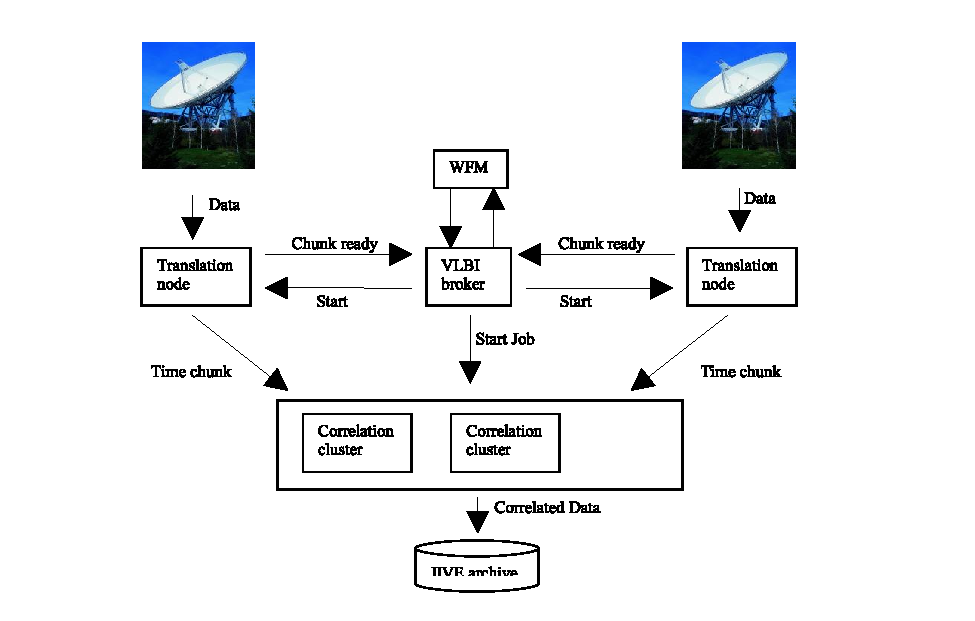
\includegraphics[width=15cm, angle=0]{figures/grid.eps}
\caption{Distribution at grid level.}
\end{figure} 

\begin{itemize}
\item The The Work Flow Manager (WFM) starts the correlation process. The user specifies a VEX file and the WFM converts it to a CCF file. WFM notifies VLBI Broker about the new experiment, which is responsible for managing the further process.
\item The VLBI broker starts the translation nodes, which open a connection to a telescope. 
\item The translation nodes send messages back to the broker when time chunks are available. It is the task of the translation node to buffer the data and to chop the incoming data stream into chunks.  
\item When a time chunk is available for all telescopes, the VLBI broker sends a start message to the translation and the correlation nodes. The translation nodes send the data to the correlation clusters which do the processing.
\item After the correlation of the chunk the output of all time chunks is transferred to a central location from which JIVE can retrieve the data using grid FTP
\end{itemize}


\section{Web Service}\label{webservice}

This document is not about explaining the details of WSDL, SOAP, ZSI package etc. 
Please see references to see a list of documentation on these items.
We assume that ZSI package is installed and we aim on writing a web service and a client 
starting from a WSDL file.


\subsection{Generating the consumer (client)}\label{client}

Given the WSDL file the code outline is generated by using the wsdl2py and wsdl2dispatch 
tools that are included in ZSI package. As a first step invoke the following command to 
generate the client interface code:

\verb|  wsdl2py -bf file.wsdl|

Here "-b" is shorthand for "--complexType" and "-f" is for "--file". 
(To get the full list of options: wsdl2py --help). The above command will generate 
two files in the current working directory. Those files will be named after the WSDL definition name.

i.e., if the definition name is defined as: 

\verb|  <definition name='SampleService'>|

in the WSDL file than the resulting two file names will be:

\begin{enumerate}
  \item \textbf{Sample\_services.py} that contains a consumer stub. In particular, it contains:
    \begin{itemize}
      \item a Locator class. An instance of this class can be used to create an instance of a
binding through which the service can be invoked.
      \item a class for each operation that can be invoked on the server. This can be used to
construct a message to be sent to the server.
    \end{itemize}
  \item \textbf{Sample\_services\_types.py} that contains various helper classes associated
with the types defined in the WSDL.

\end{enumerate}

The -complexType parameter causes wsdl2py to generate helper methods (getters, setters
and factory methods) for each complex type in the WSDL.


\subsection{Generating the Server}\label{server}

To create the basic code for a server, the following command should then be run. Note that
wsdl2py needs to be run first.

\verb|  wsdl2dispatch --extended --file file.wsdl|

This creates the file: Sample\_services\_server.py that contains a framework for the server.









\section{Translation Node Web Service}\label{tn}

Let's continue explaining the web service on a real example. We would like to
implement the Translation Node web service. The procedure can be summarized as
follows:

\begin{itemize}
  \item Grid broker sends a request to the Translation Node service including
the necessary data
  \item Translation Node service processes and transfers the data to the
required location
  \item Translation Node service sends back a Notification message indicating
required messages
\end{itemize}

First of all let's have a look at the WSDL file that we are going to use:

\begin{verbatim}
TranslationNode.wsdl:

<wsdl:types>
  <xs:schema xmlns:xs="http://www.w3.org/2001/XMLSchema"
  attributeFormDefault="qualified" elementFormDefault="qualified"
  targetNamespace="http://tr.remote.expres.psnc.pl/xsd">
    <xs:element name="startTranslationJob">
      <xs:complexType>
        <xs:sequence>
          <xs:element name="param0" nillable="true" type="xsd:JobInfo"/>
        </xs:sequence>
      </xs:complexType>
    </xs:element>
    <xs:element name="JobInfo" type="xsd:JobInfo"/>
    <xs:complexType name="JobInfo">
      <xs:sequence>
        <xs:element name="brokerIPAddress" nillable="true" type="xs:string"/>
        <xs:element name="chunkSize" type="xs:long"/>
        <xs:element name="endTime" nillable="true" type="xs:string"/>
        <xs:element name="startTime" nillable="true" type="xs:string"/>
        <xs:element name="stationName" nillable="true" type="xs:string"/>
        <xs:element name="experimentName" nillable="true" type="xs:string"/>
      </xs:sequence>
    </xs:complexType>
  </xs:schema>
<wsdl:types>

\end{verbatim} 

Here we should pay attention that there are two "complexType"s defined under one
"schema". For more info please look at reference \cite{xmlman} for the standard
XML Schema manual or \cite{xmltut} for a detailed tutorial.

First of all we use the wsdl2py and wsdl2dispatch tools to generate the
interfaces:

\verb|  wsdl2py -bf file.wsdl|,

generates {\it TranslationNode\_services.py} and {\it
TranslationNode\_services\_types.py} files and

\verb|  wsdl2dispatch --extended --file file.wsdl|

generates the {\it TranslationNode\_services\_server.py} file.

\subsection{Client for Translation Node web service}\label{tn_client}

We should write the necessary consumer code. In this case the client needs to
send data to the service. For the complete client and service codes please see
the original codes. Below we give a more compact generic forms of these codes.

\begin{verbatim}
TranslationNodeRequest.py:

# import the generated class stubs
from TranslationNode_services import *

# create a new request
req = startTranslationJobMessage()
req.Param0 = req.new_param0()

# of course we need to read in (or define) data to be sent first
# details can be seen from the original code
req.Param0.BrokerIPAddress=brokerIPAdress
req.Param0.ChunkSize=chunkSize
req.Param0.StartTime=startTime
req.Param0.EndTime=endTime
req.Param0.StationName=stationName
req.Param0.ExperimentName=experimentName

# get a port proxy instance
# translationnode is the name of the service
# portnumber is defined in the input file
loc = TranslationNodeLocator()
serviceLocation = 'http://huygens:' + portNumber + '/translationnode'
port = loc.getTranslationNodePortType(serviceLocation)

# actualy ask the service to do the job
resp = port.startTranslationJob(req)

# print out the response
print resp
\end{verbatim}

An example of the data file is as follows:

\begin{verbatim}
experiment_data.inp:

# grid broker IP address
# where the response notification will be sent
jop32
# chunk size in bytes or "scan size"
# when "scan size", calculates the actual chunk size as the size of a scan 
10000
# port number
8082
# start time of the first chunk
2007y158d18h41m30s
# end time
2007y158d18h41m32s
# Station code (two letter name of station)
Ef
# vax file name
ez015.vix
\end{verbatim}


\subsection{Service for Translation Node web service}\label{tn_service}

The service should receive the request, do the process and
finally notice the Notification service. The process is as follows:
\begin{itemize}
  \item Receive the data from the client
  \item Calculate the actual size of the chunk
  \item Check if the requested data already downloaded from Mark5 previously
  \item If not downloaded, connect Mark5 and download requested data (disk has
to be inserted before)
  \item If files already exist then check the size of the files and if
necessary split them up with the required chunk size
  \item Copy the files over the grid ftp
  \item Notify the Notification service that the file is copied (with necessary
data)
\end{itemize}

Below is the short listing of the service:

\begin{verbatim}
TranslationNodeService.py:

#!/usr/bin/env python2.4
from ZSI.ServiceContainer import AsServer
from ZSI import ServiceProxy
from TranslationNode_services_server import *
from TranslationNode_mark5 import *
from TranslationNode_vex import *
from TranslationNodeNotification import *

# Read in or define the configuration parameters
portMark5Data = ...
portMark5Control = ...
ipMark = ...
host = ...
gridFtpIP = ...
fileName = ...
block_size = ...
portNumber = ...

class Service(TranslationNode):

  def soap_startTranslationJob(self, ps):
    """ Main service function actually starts the translation job."""
    rsp = TranslationNode.soap_startTranslationJob(self, ps)
    msg = self.request

# this is where everything is calculated...

# Information passed to us by the VLBI grid broker
    station = msg.Param0.StationName
    ...

    # Open VEX file and read in some data
    vex = Vex(str(vex_file_name))
    ...
    ...

    sched = vex['SCHED']

# within the following for loop we perform all necessary process
# please see the original code for details

    for scan in sched:

      ...
      ...

      - Calculate the actual size of the chunk

      - Check if the requested data already downloaded from Mark5 previously

      - If not downloaded, connect Mark5 and download requested data (disk has
to be inserted before)

      - If files already exist then check the size of the files and if
necessary split them up with the required chunk size

      - Copy the files over the grid ftp

      ...
      ...

# After the file is splitted or downloaded than notify the grid broker
# The host name below belongs to the host of the Notification service
        print "send notification to grid broker..."
        node_notification = TranslationNodeNotification(host,
                                                        10001,
                                                        gridFtpIP,
                                                        chunk_real_size,
                                                        chunk_end,
                                                        chunk_start,
                                                        "http://huygens",
                                                        20001)

      ...
      ...

      continue

# end of calculation

    return rsp

# The following lines actually starts the service
# the service name is defined here as Service('servicename')
# This service is run at: http://url-of-the-machine:portnumber/servicename
if __name__ == "__main__" :
  port = portNumber
  AsServer(port, (Service('translationnode'),))

\end{verbatim}

and the corresponding input files is:

\begin{verbatim}
mark5_connect_data.inp:

# Data socket number
2630
#Control socket number
2620
# Mark5 IP address
192.42.120.6
# IP address of the machine where the service is run
192.42.120.69
# grid ftp address where the file is to be transfered
# this adress has to be the full path to the directory
# i.e. relative to a home directory : melisa.man.poznan.pl/~/
# i.e. absolute path: huygens.nfra.nl/data4/sfxc/
#huygens.nfra.nl/data4/sfxc/huseyin/tn/junk_mark5/
melisa.man.poznan.pl/~/
# path to download/copy files to
/data4/sfxc/huseyin/tn/download_mark5/
# block size
8192
# port number
8082
\end{verbatim}
\subsection{Client for Translation Node Notification web
service}\label{tn_notification}

As we have mentioned earlier the Translation Node service sends a notification
to the Notification service after it processes the request. For the mentioned
notification that part of the Translation Node service acts as a client. Since
there are some differences between the Translation Node service and the
Notification service, it would be a good idea to give the details of
Notification service as well.

First of all let's have a look at the corresponding WSDL file of the
Notification service:

\begin{verbatim}
TranslationNodeNotification.wsdl:

  <wsdl:types>
    <xs:schema attributeFormDefault="qualified" elementFormDefault="qualified"
targetNamespace="http://broker.remote.expres.psnc.pl/xsd"
xmlns:xsd="http://broker.remote.expres.psnc.pl/xsd">
    <xs:element name="chunkIsReady">
        <xs:complexType>
            <xs:sequence>
                <xs:element minOccurs="0" name="param0" nillable="true"
type="ns1:ChunkInfo"/>
            </xs:sequence>
        </xs:complexType>
    </xs:element>
</xs:schema>
    <xs:schema attributeFormDefault="qualified" elementFormDefault="qualified"
targetNamespace="http://jobinfo.broker.remote.expres.psnc.pl/xsd"
xmlns:ax21="http://jobinfo.broker.remote.expres.psnc.pl/xsd">
    <xs:complexType name="ChunkInfo">
        <xs:sequence>
            <xs:element minOccurs="0" name="chunkId" type="xs:long"/>
            <xs:element minOccurs="0" name="chunkLocation" nillable="true"
type="xs:string"/>
            <xs:element minOccurs="0" name="chunkSize" type="xs:long"/>
            <xs:element minOccurs="0" name="endTime" nillable="true"
type="xs:string"/>
            <xs:element minOccurs="0" name="startTime" nillable="true"
type="xs:string"/>
            <xs:element minOccurs="0" name="translationNodeIP" nillable="true"
type="xs:string"/>
            <xs:element minOccurs="0" name="translationNodeId" type="xs:int"/>
        </xs:sequence>
    </xs:complexType>
</xs:schema>
  </wsdl:types>
\end{verbatim}

When we compare the above WSDL file with the TranslationNode.wsdl we see that
here the complexType and it's elements span different name spaces and
defined in different schemas while they span the same name space and defined i
n the same schema in the previous WSDL file. After generating the interface
classes from this WSDL file with wsdl2py and wsdl2dispatch tools, as explained
above, we will also see differences in *\_services\_types.py files. A closer
look at the TranslationNodeNotification\_services\_types.py reveals that there
are two separete classes (ns0 and ns1) are generated for this case where there
was only one class (ns0) is generated for TranslationNode.wsdl file.

Keeping in mind the above differences, we should implement the client code
accordingly:

\begin{verbatim}
TranslationNodeNotification.wsdl: (client for Notification service)

import sys
from TranslationNodeNotification_services import *

class TranslationNodeNotification:
  def __init__(self):
    self.resp_list=[]

  def __init__(self, BrokerIPAdress=None, 
               chunkId = None, 
               chunkLocation = None, 
               chunkSize = None, 
               endTime = None, 
               startTime = None, 
               translationNodeIP = None, 
               translationNodeId = None):
    
    """ This is a TranslationNodeNotification service simulator. 
    This service is used to test if the TranslationNodeService is sending
    the notification correctly after the downloading/copying from Mark5 
    operations are finished. """
    
# define request
    req = chunkIsReadyRequest()
    req.Param0 = req.new_param0()  

# assign parameters to be sent (received from TranslationNodeService.py)
    req.Param0.ChunkId = chunkId
    req.Param0.ChunkLocation = chunkLocation
    req.Param0.ChunkSize = chunkSize
    req.Param0.EndTime = endTime
    req.Param0.StartTime = startTime
    req.Param0.TranslationNodeIP = translationNodeIP
    req.Param0.TranslationNodeId = translationNodeId

# Those parameters can be accessed here as follows:
    print 'chunk ID: ', req.Param0.ChunkId

# get a port proxy instance
    loc = TranslationNodeNotificationLocator()
    locationName =
'http://melisa.man.poznan.pl:8080/axis2/services/TranslationNodeNotification'
# tracefile=sys.stdout parameter prints the sent request on the screen
    port = loc.getTranslationNodeNotificationPortType(locationName,
tracefile=sys.stdout)

# actualy ask the service to do the job
    resp = port.chunkIsReady(req)
\end{verbatim}

The complete listings of the above codes together with the grid broker service
and client simulators are included as an appendix.
\section{Running the web service}\label{running}

Since we are going to copy the data over a grid ftp we need to set up and
intiate the grid ftp server first. Assumed that Globus is installed:

\begin{itemize}
\item log in as jops (to i.e. huygens) and set up the Globus environment with
either: \\
  \verb|  $ setenv GLOBUS_LOCATION /huygens_1/jops/globus| \\
  \verb|  $ source $GLOBUS_LOCATION/etc/globus-user-env.csh| \\
or: \\
  \verb|  $ export GLOBUS_LOCATION=/huygens_1/jops/globus| \\
  \verb|  $ . $GLOBUS_LOCATION/etc/globus-user-env.sh|
\item Now, you can start the server (as user jops) by: \\
  \verb|  $ grid-proxy-init -key /etc/grid-security/containerkey.pem -cert \|\\
  \verb|    /etc/grid-security/containercert.pem| \\
  \verb|  $ globus-gridftp-server -p 2811|
\item After that, you can log in as yourself and set up the environment as
above.  Make sure that you have a ~/.globus directory with your
private key (userkey.pem) and your certificate.(usercert.pem, which
you got by mail).  If that's the case, you should be able to create a
proxy certificate using: \\
  \verb|  $ grid-proxy-init| \\
This will ask you to enter the passphrase for your key.
\item You should be able to use the GridFTP client:\\
  \verb|  $ globus-url-copy gsiftp://huygens.nfra.nl/SRC file://DEST|
\item Now you are ready to run the web service:
  \verb|  python TranslationNodeService.py|
\end{itemize}

More documentation can be found at:\\
  \verb|  http://www.globus.org/toolkit/docs/4.0/data/gridftp/|






\appendix
\section{Code Listings}\label{codes}

\subsection{TranslationNodeRequest.py}
\begin{verbatim}
from TranslationNode_services import *
# we need to skip comments in input file.
# For that we make use of re
import re

# define comment characters
comment_char = re.compile(r'^\s*#')

# define a list and initialize it with anything and don't use inp[0] later on 
inp = ['##']
# if the first character matches the comment character skip that line
# otherwise read the line
fileExp = file('experiment_data.inp')
for line in fileExp:
  if comment_char.match(line):
    continue
  inp.append(line)

# we are done with reading. we can close the file
fileExp.close()

# define request
req = startTranslationJobMessage()
req.Param0 = req.new_param0()  

# get broker ip address from the read file
req.Param0.BrokerIPAddress=inp[1].strip()

# get chunk size to read in from the read file
bytes_string = inp[2]
bytes = bytes_string.strip()

# get port number from the read file
portNumber_string = inp[3]
portNumber = portNumber_string.strip()

# test if the http address correctly parsed
loc = TranslationNodeLocator()
portTest = 'http://huygens:' + portNumber + '/translationnode'
print portTest
port = loc.getTranslationNodePortType(portTest)

# initialize the chunk size
if (bytes == "scan size"):
  req.Param0.ChunkSize=0
else: 
  req.Param0.ChunkSize=eval(bytes) 

# read the rest of the parameters from the read file
req.Param0.StartTime=inp[4].strip()
req.Param0.EndTime=inp[5].strip()
req.Param0.StationName=inp[6].strip()
req.Param0.ExperimentName=inp[7].strip()

print "broker IP address ", req.Param0.BrokerIPAddress
print "bytes ", bytes
print "portNumber ", portNumber
print "chunksize ", req.Param0.ChunkSize
print "Start time ", req.Param0.StartTime
print "End time ", req.Param0.EndTime
print "Station name ", req.Param0.StationName
print "Experiment name ", req.Param0.ExperimentName

# actualy ask the service to do the job
resp = port.startTranslationJob(req)
\end{verbatim} 

\subsection{experiment\_data.inp}
\begin{verbatim}
# grid broker IP address
# where the response notification will be sent
jop32
# chunk size in bytes or "scan size"
# when "scan size", calculates the actual chunk size as the size of a scan 
10000
# port number
8082
# start time of the first chunk
2007y158d18h41m30s
# end time
2007y158d18h41m32s
# Station code (two letter name of station)
Ef
# vax file name
ez015.vix
\end{verbatim} 

\subsection{TranslationNodeService.py}
\begin{verbatim}
#!/usr/bin/env python2.4
import sys
import time
import os
from os.path import join, getsize, exists, split
from ZSI.ServiceContainer import AsServer
from ZSI import ServiceProxy
from TranslationNode_services_server import *
from TranslationNode_mark5 import *
from TranslationNode_vex import *
from TranslationNodeNotification import *
# we need to skip comments in input file.
# For that we make use of re
import re

# define comment characters
comment_char = re.compile(r'^\s*#')

# define a list and initialize it with anything and don't use inp[0] later on 
inp = ['##']
# if the first character matches the comment character skip that line
# otherwise read the line
for line in file('mark5_connect_data.inp'):
  if comment_char.match(line):
    continue
  inp.append(line)

# read in the Data port number
portMark5Data = int(inp[1].strip())

# read in the Control port number
portMark5Control = int(inp[2].strip())

# IP address of the Mark5 that will be connected
ipMark = inp[3].strip()

# IP address of the host where the service is run
host = inp[4].strip()

# url address of the grid ftp 
#including the location of the directory where the files to be copied
gridFtpIP = inp[5].strip()

# file path that the data will be copied to
fileName = inp[6].strip()
fileName = fileName.strip()

# read in the block size
block_size = int(inp[7].strip())

# port number 
portNumber = int(inp[8].strip())

class Service(TranslationNode):

  def soap_startTranslationJob(self, ps):
    """ Main service function actually starts the translation job."""
    rsp = TranslationNode.soap_startTranslationJob(self, ps)
    msg = self.request
    print 'Requested broker IP address: ', msg.Param0.BrokerIPAddress
    print 'Requested start time: ', msg.Param0.StartTime
    print 'Requested end time: ', msg.Param0.EndTime
    print 'Requested chunk size: ', msg.Param0.ChunkSize
    print 'Requested station name: ', msg.Param0.StationName
    print 'Requested experiment name: ', msg.Param0.ExperimentName

# this is where everything is calculated...

#		Mark5_connect(portMark5Data, portMark5Control, ipMark) 

# Information passed to us by the VLBI grid broker
    station = msg.Param0.StationName
    brokerIP = msg.Param0.BrokerIPAddress
    chunk_size = msg.Param0.ChunkSize
    job_start = parse_vex_time(msg.Param0.StartTime)
    job_end = parse_vex_time(msg.Param0.EndTime)
    vex_file_name = msg.Param0.ExperimentName
    vex_file_name = vex_file_name.strip()
    experiment_name = vex_file_name.split('.')
#		print "experiment_name ==> '"+str(type(vex_file_name))-+"'"
    
    print 'host IP address: ', host
    print 'broker address: ', brokerIP
    
    # Open VEX file
    vex = Vex(str(vex_file_name))

    chunk_start = job_start
    chunk_time = job_start
    start_scan = None

    sched = vex['SCHED']
    chunk_number = 0
    for scan in sched:
      if not start_scan:
        start_scan = scan
        pass
      scan_start = parse_vex_time(sched[scan]['start'])

      if scan_start > chunk_time:
        chunk_time = scan_start

      data_format = vex.get_data_format(scan, station)
      overhead = data_format_overhead[data_format]

# Find out the true length of the scan, which is just the maximum
# of the per-station length of the scan.
      secs = 0
      for info in sched[scan].getall('station'):
        secs = max(secs, info[2])
        continue
      scan_end = scan_start + float(secs.split()[0])

# If the this scan ends before the job starts, skip it.
      if scan_end < job_start:
        continue
      if scan_start > job_end:
        continue

# Calculate the data rate for this scan.
# Calculated the size of a chunk that fits in to 1 second
# make sure that the chunk size is at least equals to 1 second data size
# if required chunk size corresponds to a floating point seconds use int value
      mode = vex.get_mode(scan)
      bits_per_sample = vex.get_bits_per_sample(mode, station)
      num_channels = vex.get_num_channels(mode, station)
      sample_rate = vex.get_sample_rate(mode, station)
      data_rate = num_channels * sample_rate * bits_per_sample * overhead

      if (msg.Param0.ChunkSize == 0):
        chunk_size=(scan_end - scan_start)*(data_rate/8)

      chunk_to_data_rate = int(chunk_size / (data_rate/8))

      if chunk_to_data_rate == 0:
        chunk_to_data_rate += 1

      chunk_size = chunk_to_data_rate * (data_rate/8)
      chunk_bytes = chunk_size

# set head position on the disk on Mark5
      start_position = float(vex.get_data_start(scan, station))
      start_position = int(start_position*1000*1000*1000)
      mark5_set_output = Mark5_set_position()
      time_real_start = mark5_set_output.bytes_starting_position(host,
portMark5Data, portMark5Control, ipMark, start_position)
      time_real_start_ms = re.search("\.(\d{4})s", time_real_start)
      time_real_start_ms = float("0."+time_real_start_ms.group(1))
      time_real_start=re.sub("\.\d*", "", time_real_start)
      time_real_start=parse_vex_time(time_real_start)
      if (job_start > scan_start):
        time_start_diff = time_real_start-job_start
      else:
        time_start_diff = time_real_start-scan_start
      bytes_starting_diff = (time_start_diff+time_real_start_ms)*(data_rate/8)

# Chop it up and chunks 
      chunk_end = chunk_time + chunk_size / (data_rate / 8)
      chunk_end = min(chunk_end, job_end)
      chunk_start_check = max(job_start, scan_start)
      
      chunk_real_end_size_temp = (scan_end-scan_start) * (data_rate / 8) /
chunk_size
      chunk_real_end_size = (chunk_real_end_size_temp -
int(chunk_real_end_size_temp))*chunk_size
      if chunk_real_end_size ==0:
        chunk_real_end_size = chunk_size
      scan_size = (scan_end-scan_start)*(data_rate/8)
      
      while chunk_end <= scan_end:
        print "chunk", chunk_number, scan, \
          strftime("%Yy%jd%Hh%Mm%Ss", localtime(chunk_start)), scan, \
          strftime("%Yy%jd%Hh%Mm%Ss", localtime(chunk_end))

# Consider several conditions to deliver the right chunk
        if (time_real_start > chunk_start_check and
int(bytes_starting_diff/chunk_size)>0):
          chunk_real_size=0
        elif (time_real_start >= chunk_start_check and
int(bytes_starting_diff/chunk_size)==0):
          chunk_real_size=chunk_size - time_real_start_ms * (data_rate / 8)
        elif (chunk_end == scan_end):
          chunk_real_size = chunk_real_end_size
        elif ((chunk_end-chunk_start)*(data_rate/8) < chunk_size):
          chunk_real_size=(chunk_end-chunk_start)*(data_rate/8)
        else :
          chunk_real_size=chunk_size

        chunk_diff=chunk_end-chunk_start
        chunk_diff_size = chunk_diff*(data_rate/8)

        chunk_start_check=chunk_end

# give a logical name to the file that is downloaded from Mark5
        sendFile = experiment_name[0] + '_' + station + '_' + str(scan) + "_" +
str(chunk_number) + '.m5a'
        sendFile = fileName + sendFile.lower()
        print "file to be sent: " + sendFile

#  If file is already downloaded from Mark5 before, we don't need to download it
again
#  just split the existing file in to required chunk size and send it
        if exists(sendFile):
          file_size =  getsize(sendFile)

        if (exists(sendFile) and file_size > 0):
          print "file size = " + str(file_size)
          print "chunk size = " + str(chunk_bytes)
          if (file_size <= chunk_bytes):
# please note: If the gridftp server is not started yet, the following operation
will fail
            copyFile = "globus-url-copy file://" + str(sendFile) + " gsiftp://"
+ gridFtpIP
            print copyFile
            os.system(copyFile)
          elif (file_size > chunk_bytes):
            split_command = "split -d -a 3 -b " + str(int(chunk_bytes)) + " " +
sendFile + " " + sendFile
            os.system(split_command)
            nr_files = file_size/chunk_bytes + 1
            i=0
# include leading zeros tot he file names accordingly
            while i < nr_files:
              if nr_files <= 9:
                filename2 = sendFile + "00" + str(i)
              elif (nr_files >9 and nr_files <= 99):
                filename2 = sendFile + "0" + str(i)
              elif (nr_files >99 and nr_files <= 999):
                filename2 = sendFile + str(i)

            print filename2
# please note: If the gridftp server is not started yet, the following operation
will fail
            copyFile = "globus-url-copy file://" + str(filename2) + " gsiftp://"
+ gridFtpIP
            print copyFile
            os.system(copyFile)
            i +=1
            continue
        elif (exists(sendFile) and file_size == 0):
          break
        else:
# If file doesn't already exist than download it from Mark5
          mark5_chunk_output = Mark5_get_chunks(host, 
          portMark5Data,
          portMark5Control, 
          ipMark, 
          sendFile, 
          block_size, 
          chunk_real_size, 
          start_position)
          print mark5_chunk_output

        time.sleep(1)

# After the file is splitted or downloaded than notify the grid broker
# The host name below belongs to the host of the Notification service
        print "send notification to grid broker..."
        node_notification = TranslationNodeNotification(host,
                                                        10001,
                                                        gridFtpIP,
                                                        chunk_real_size,
                                                        chunk_end,
                                                        chunk_start,
                                                        "http://huygens",
                                                        20001)

        print node_notification
        print "end of notification to grid broker..."

        if chunk_end >= job_end:
          break

        if chunk_end >= scan_end:
          break

        chunk_start = chunk_time = chunk_end
        chunk_end = chunk_time + chunk_size / (data_rate / 8)
        if scan_end < job_end:
          chunk_end = min(chunk_end, scan_end)
        elif scan_end >= job_end:
          chunk_end = min(chunk_end, job_end)

        chunk_bytes = chunk_size
        chunk_number += 1
        start_scan = scan
        continue

      chunk_time = scan_end
      chunk_start = chunk_time
      chunk_bytes = chunk_size
      chunk_number += 1
      start_scan = scan
      chunk_bytes -= (scan_end - scan_start) * (data_rate / 8)
      chunk_number = 0
      continue



# end of calculation
# Mark5_disconnect()
    return rsp

# The following lines actually starts the service
# the service name is defined here as Service('servicename')
# This service is run at: http://url-of-the-machine:portnumber/servicename
if __name__ == "__main__" :
  port = portNumber
  AsServer(port, (Service('translationnode'),))
\end{verbatim} 

\subsection{mark5\_connect\_data.inp}
\begin{verbatim}
# Data socket number
2630
#Control socket number
2620
# Mark5 IP address
192.42.120.6
# IP address of the machine where the service is run
192.42.120.69
# grid ftp address where the file is to be transfered
# this adress has to be the full path to the directory
# i.e. relative to a home directory : melisa.man.poznan.pl/~/
# i.e. absolute path: huygens.nfra.nl/data4/sfxc/
#huygens.nfra.nl/data4/sfxc/huseyin/tn/junk_mark5/
melisa.man.poznan.pl/~/
# path to download/copy files to
/data4/sfxc/huseyin/tn/download_mark5/
# block size
8192
# port number
8082
\end{verbatim} 

\begin{verbatim}
TranslationNodeNotification.py:

import sys
from TranslationNodeNotification_services import *

class TranslationNodeNotification:
  def __init__(self):
    self.resp_list=[]

  def __init__(self, BrokerIPAdress=None, 
               chunkId = None, 
               chunkLocation = None, 
               chunkSize = None, 
               endTime = None, 
               startTime = None, 
               translationNodeIP = None, 
               translationNodeId = None):
    
    """ This is a TranslationNodeNotification service simulator. 
    This service is used to test if the TranslationNodeService is sending
    the notification correctly after the downloading/copying from Mark5 
    operations are finished. """
    
  # define request
    req = chunkIsReadyRequest()
    req.Param0 = req.new_param0()  

  # get broker ip address from the read file
#    req.Param0.BrokerIPAddress = BrokerIPAddress
    req.Param0.ChunkId = chunkId
    req.Param0.ChunkLocation = chunkLocation
    req.Param0.ChunkSize = chunkSize
    req.Param0.EndTime = endTime
    req.Param0.StartTime = startTime
    req.Param0.TranslationNodeIP = translationNodeIP
    req.Param0.TranslationNodeId = translationNodeId


    print 'chunk ID: ', req.Param0.ChunkId
    print 'chunk Location: ', req.Param0.ChunkLocation
    print 'Requested chunk size: ', req.Param0.ChunkSize
    print 'Requested end time: ', req.Param0.EndTime
    print 'Requested start time: ', req.Param0.StartTime
    print 'translationNode IP: ', req.Param0.TranslationNodeIP
    print 'translationNode Id: ', req.Param0.TranslationNodeId

  # get port number from the read file
    portNumber_string = "8080"
    portNumber = portNumber_string.strip()
    print portNumber

  # test if the http address correctly parsed
    loc = TranslationNodeNotificationLocator()
    #portTest = 'http://jop32:' + portNumber + '/notification'
    portTest =
'http://melisa.man.poznan.pl:8080/axis2/services/TranslationNodeNotification'
    print portTest
    port = loc.getTranslationNodeNotificationPortType(portTest,
tracefile=sys.stdout)

  # actualy ask the service to do the job
    resp = port.chunkIsReady(req)
\end{verbatim} 

\subsection{gridBrokerRequestSimulator.py}
\begin{verbatim}
import sys
from TranslationNodeNotification_services import *

# define request
req = chunkIsReadyRequest()
req.Param0 = req.new_param0()

# get broker ip address from the read file
# actually both declaration types work
# declaring i.e. req.chunkId=0 wouldn't work
req.Param0.ChunkId = 10001
req.Param0.set_element_chunkLocation("huygens/data4/")
req.Param0.set_element_chunkSize(123456)
req.Param0.set_element_endTime("2007y158d18h59m00s")
req.Param0.set_element_startTime("2007y158d18h56m00s")
req.Param0.set_element_translationNodeIP("192.42.120.22")
req.Param0.set_element_translationNodeId(20001)

# get port number from the read file
portNumber_string = "8080"
portNumber = portNumber_string.strip()
print portNumber

# test if the http address correctly parsed
# get a port proxy instance
#http://melisa.man.poznan.pl:8080/axis2/services/TranslationNodeNotification
loc = TranslationNodeNotificationLocator()
#portTest = 'http://jop32:' + portNumber + '/notification'
portTest = 'http://melisa.man.poznan.pl:' + portNumber +
'/axis2/services/TranslationNodeNotification'
print portTest
port = loc.getTranslationNodeNotificationPortType(portTest,
tracefile=sys.stdout)

# Note that both of the following implementations work
print "Chunk Id", req.Param0.get_element_chunkId()
print "Chunk Location", req.Param0.ChunkLocation

# actualy ask the service to do the job
resp = port.chunkIsReady(req)
print resp
\end{verbatim} 

\subsection{gridBrokerServiceSimulator.py}
\begin{verbatim}
#!/usr/bin/env python2.4
from ZSI.ServiceContainer import AsServer
from ZSI import ServiceProxy
from TranslationNodeNotification_services_server import *

class Service(TranslationNodeNotification):
  def soap_chunkIsReady(self, ps):
    rsp = TranslationNodeNotification.soap_chunkIsReady(self, ps)
    msg = self.request

    print "hello Mark..."
    print 'chunk ID: ', msg.Param0.get_element_chunkId()
    print 'chunk Location: ', msg.Param0.get_element_chunkLocation()
    print 'Requested chunk size: ', msg.Param0.get_element_chunkSize()
    print 'Requested end time: ', msg.Param0.get_element_endTime()
    print 'Requested start time: ', msg.Param0.get_element_startTime()
    print 'translationNode IP: ', msg.Param0.get_element_translationNodeIP()
    print 'translationNode Id: ', msg.Param0.get_element_translationNodeId()
        
    return rsp

if __name__ == "__main__" :
  port = 8080
  AsServer(port, (Service('notification'),))
\end{verbatim} 

\begin{verbatim}
TranslationNode.wsdl:

<wsdl:definitions xmlns:soap12="http://schemas.xmlsoap.org/wsdl/soap12/"
xmlns:http="http://schemas.xmlsoap.org/wsdl/http/"
xmlns:mime="http://schemas.xmlsoap.org/wsdl/mime/"
xmlns:xsd="http://tr.remote.expres.psnc.pl/xsd"
xmlns:soap="http://schemas.xmlsoap.org/wsdl/soap/"
xmlns:wsdl="http://schemas.xmlsoap.org/wsdl/"
xmlns:nsTr="http://tr.remote.expres.psnc.pl"
targetNamespace="http://tr.remote.expres.psnc.pl">
	<wsdl:types>
		<xs:schema xmlns:xs="http://www.w3.org/2001/XMLSchema"
attributeFormDefault="qualified" elementFormDefault="qualified"
targetNamespace="http://tr.remote.expres.psnc.pl/xsd">
			<xs:element name="startTranslationJob">
				<xs:complexType>
					<xs:sequence>
						<xs:element name="param0"
nillable="true" type="xsd:JobInfo"/>
					</xs:sequence>
				</xs:complexType>
			</xs:element>
			<xs:element name="JobInfo" type="xsd:JobInfo"/>
			<xs:complexType name="JobInfo">
				<xs:sequence>
					<xs:element name="brokerIPAddress"
nillable="true" type="xs:string"/>
					<xs:element name="chunkSize"
type="xs:long"/>
					<xs:element name="endTime"
nillable="true" type="xs:string"/>
					<xs:element name="startTime"
nillable="true" type="xs:string"/>
					<xs:element name="stationName"
nillable="true" type="xs:string"/>
					<xs:element name="experimentName"
nillable="true" type="xs:string"/>
				</xs:sequence>
			</xs:complexType>
		</xs:schema>
	</wsdl:types>
	<wsdl:message name="startTranslationJobMessage">
		<wsdl:part name="part1" element="xsd:startTranslationJob"/>
	</wsdl:message>
	<wsdl:portType name="TranslationNodePortType">
		<wsdl:operation name="startTranslationJob">
			<wsdl:input message="nsTr:startTranslationJobMessage"
xmlns:wsaw="http://www.w3.org/2006/05/addressing/wsdl"
wsaw:Action="urn:startTranslationJob"/>
		</wsdl:operation>
	</wsdl:portType>
	<wsdl:binding name="TranslationNodeSOAP11Binding"
type="nsTr:TranslationNodePortType">
		<soap:binding style="document"
transport="http://schemas.xmlsoap.org/soap/http"/>
		<wsdl:operation name="startTranslationJob">
			<soap:operation soapAction="urn:startTranslationJob"
style="document"/>
			<wsdl:input>
				<soap:body use="literal"/>
			</wsdl:input>
		</wsdl:operation>
	</wsdl:binding>
	<wsdl:binding name="TranslationNodeSOAP12Binding"
type="nsTr:TranslationNodePortType">
		<soap12:binding transport="http://schemas.xmlsoap.org/soap/http"
style="document"/>
		<wsdl:operation name="startTranslationJob">
			<soap12:operation soapAction="urn:startTranslationJob"
style="document"/>
			<wsdl:input>
				<soap12:body use="literal"/>
			</wsdl:input>
		</wsdl:operation>
	</wsdl:binding>
	<wsdl:service name="TranslationNode">
		<wsdl:port name="TranslationNodeSOAP11port"
binding="nsTr:TranslationNodeSOAP11Binding">
			<soap:address
location="http://localhost:8080/axis2/services/TranslationNode"/>
		</wsdl:port>
		<wsdl:port name="TranslationNodeSOAP12port"
binding="nsTr:TranslationNodeSOAP12Binding">
			<soap12:address
location="http://localhost:8080/axis2/services/TranslationNode"/>
		</wsdl:port>
	</wsdl:service>
</wsdl:definitions>
\end{verbatim} 

\begin{verbatim}
TranslationNodeNotification.py:

<?xml version="1.0" encoding="UTF-8"?>
<wsdl:definitions targetNamespace="http://broker.remote.expres.psnc.pl"
xmlns:axis2="http://broker.remote.expres.psnc.pl"
xmlns:soap12="http://schemas.xmlsoap.org/wsdl/soap12/"
xmlns:ns0="http://broker.remote.expres.psnc.pl/xsd"
xmlns:mime="http://schemas.xmlsoap.org/wsdl/mime/"
xmlns:http="http://schemas.xmlsoap.org/wsdl/http/"
xmlns:ns1="http://jobinfo.broker.remote.expres.psnc.pl/xsd"
xmlns:wsaw="http://www.w3.org/2006/05/addressing/wsdl"
xmlns:xs="http://www.w3.org/2001/XMLSchema"
xmlns:soap="http://schemas.xmlsoap.org/wsdl/soap/"
xmlns:wsdl="http://schemas.xmlsoap.org/wsdl/">
  <wsdl:types>
    <xs:schema attributeFormDefault="qualified" elementFormDefault="qualified"
targetNamespace="http://broker.remote.expres.psnc.pl/xsd"
xmlns:xsd="http://broker.remote.expres.psnc.pl/xsd">
    <xs:element name="chunkIsReady">
        <xs:complexType>
            <xs:sequence>
                <xs:element minOccurs="0" name="param0" nillable="true"
type="ns1:ChunkInfo"/>
            </xs:sequence>
        </xs:complexType>
    </xs:element>
</xs:schema>
    <xs:schema attributeFormDefault="qualified" elementFormDefault="qualified"
targetNamespace="http://jobinfo.broker.remote.expres.psnc.pl/xsd"
xmlns:ax21="http://jobinfo.broker.remote.expres.psnc.pl/xsd">
    <xs:complexType name="ChunkInfo">
        <xs:sequence>
            <xs:element minOccurs="0" name="chunkId" type="xs:long"/>
            <xs:element minOccurs="0" name="chunkLocation" nillable="true"
type="xs:string"/>
            <xs:element minOccurs="0" name="chunkSize" type="xs:long"/>
            <xs:element minOccurs="0" name="endTime" nillable="true"
type="xs:string"/>
            <xs:element minOccurs="0" name="startTime" nillable="true"
type="xs:string"/>
            <xs:element minOccurs="0" name="translationNodeIP" nillable="true"
type="xs:string"/>
            <xs:element minOccurs="0" name="translationNodeId" type="xs:int"/>
        </xs:sequence>
    </xs:complexType>
</xs:schema>
  </wsdl:types>
  <wsdl:message name="chunkIsReadyRequest">
    <wsdl:part name="parameters" element="ns0:chunkIsReady">
    </wsdl:part>
  </wsdl:message>
  <wsdl:portType name="TranslationNodeNotificationPortType">
    <wsdl:operation name="chunkIsReady">
      <wsdl:input message="axis2:chunkIsReadyRequest"
wsaw:Action="urn:chunkIsReady">
    </wsdl:input>
    </wsdl:operation>
  </wsdl:portType>
  <wsdl:binding name="TranslationNodeNotificationSOAP12Binding"
type="axis2:TranslationNodeNotificationPortType">
    <soap12:binding style="document"
transport="http://schemas.xmlsoap.org/soap/http"/>
    <wsdl:operation name="chunkIsReady">
      <soap12:operation soapAction="urn:chunkIsReady" style="document"/>
      <wsdl:input>
        <soap12:body use="literal"/>
      </wsdl:input>
    </wsdl:operation>
  </wsdl:binding>
  <wsdl:binding name="TranslationNodeNotificationHttpBinding"
type="axis2:TranslationNodeNotificationPortType">
    <http:binding verb="POST"/>
    <wsdl:operation name="chunkIsReady">
      <http:operation location="TranslationNodeNotification/chunkIsReady"/>
      <wsdl:input>
        <mime:content part="chunkIsReady" type="text/xml"/>
      </wsdl:input>
    </wsdl:operation>
  </wsdl:binding>
  <wsdl:binding name="TranslationNodeNotificationSOAP11Binding"
type="axis2:TranslationNodeNotificationPortType">
    <soap:binding style="document"
transport="http://schemas.xmlsoap.org/soap/http"/>
    <wsdl:operation name="chunkIsReady">
      <soap:operation soapAction="urn:chunkIsReady" style="document"/>
      <wsdl:input>
        <soap:body use="literal"/>
      </wsdl:input>
    </wsdl:operation>
  </wsdl:binding>
  <wsdl:service name="TranslationNodeNotification">
    <wsdl:port name="TranslationNodeNotificationSOAP12port_http"
binding="axis2:TranslationNodeNotificationSOAP12Binding">
      <soap12:address
location="http://localhost:8080/axis2/services/TranslationNodeNotification"/>
    </wsdl:port>
    <wsdl:port name="TranslationNodeNotificationHttpport"
binding="axis2:TranslationNodeNotificationHttpBinding">
      <http:address
location="http://localhost:8080/axis2/services/TranslationNodeNotification"/>
    </wsdl:port>
    <wsdl:port name="TranslationNodeNotificationSOAP11port_http"
binding="axis2:TranslationNodeNotificationSOAP11Binding">
      <soap:address
location="http://localhost:8080/axis2/services/TranslationNodeNotification"/>
    </wsdl:port>
  </wsdl:service>
</wsdl:definitions>
\end{verbatim} 



\begin{thebibliography}{99}

\bibitem{dj14} Oerlemans, R.H.J., {\it Correlator Design Specifications}, JRA1, FABRIC, WP2.2.1, deliverable DJ1.4 (also at \\ http://www.jive.nl/dokuwiki/lib/exe/fetch.php/fabric:dj1.4\_correlatordesignspecifications.doc? $\backslash$ id=fabric\%3Awp2\_distributed\_correlation\&cache=cache)
\bibitem{zsi} Salz, R., {\it ZSI: The Zolera Soap Infrastructure}, http://pywebsvcs.sourceforge.net/zsi.html
\bibitem{pyweb} {\it Python Web Services Project}, http://pywebsvcs.sourceforge.net/
\bibitem{xmlman} {\it XML Schema}, http://www.w3.org/XML/Schema
\bibitem{xmltut} {\it XML Schema Tutorial}, http://www.w3schools.com/schema/

\end{thebibliography}



%\begin{thebibliography}{99}

\bibitem{dj14} Oerlemans, R.H.J., {\it Correlator Design Specifications}, JRA1, FABRIC, WP2.2.1, deliverable DJ1.4 (also at \\ http://www.jive.nl/dokuwiki/lib/exe/fetch.php/fabric:dj1.4\_correlatordesignspecifications.doc? $\backslash$ id=fabric\%3Awp2\_distributed\_correlation\&cache=cache)
\bibitem{zsi} Salz, R., {\it ZSI: The Zolera Soap Infrastructure}, http://pywebsvcs.sourceforge.net/zsi.html
\bibitem{pyweb} {\it Python Web Services Project}, http://pywebsvcs.sourceforge.net/
\bibitem{xmlman} {\it XML Schema}, http://www.w3.org/XML/Schema
\bibitem{xmltut} {\it XML Schema Tutorial}, http://www.w3schools.com/schema/

\end{thebibliography}

% Bibliography
%
%\bibliography{thesis}
%\begin{thebibliography}{99}

\bibitem{dj14} Oerlemans, R.H.J., {\it Correlator Design Specifications}, JRA1, FABRIC, WP2.2.1, deliverable DJ1.4 (also at \\ http://www.jive.nl/dokuwiki/lib/exe/fetch.php/fabric:dj1.4\_correlatordesignspecifications.doc? $\backslash$ id=fabric\%3Awp2\_distributed\_correlation\&cache=cache)
\bibitem{zsi} Salz, R., {\it ZSI: The Zolera Soap Infrastructure}, http://pywebsvcs.sourceforge.net/zsi.html
\bibitem{pyweb} {\it Python Web Services Project}, http://pywebsvcs.sourceforge.net/
\bibitem{xmlman} {\it XML Schema}, http://www.w3.org/XML/Schema
\bibitem{xmltut} {\it XML Schema Tutorial}, http://www.w3schools.com/schema/

\end{thebibliography}


%
\end{document}
